
%----------------------------------------------------------------------------------------
%	Machine Learning Assignment Template
%----------------------------------------------------------------------------------------

\documentclass[11pt]{scrartcl}
\newcommand*\student[1]{\newcommand{\thestudent}{{#1}}}

%----------------------------------------------------------------------------------------
%	INSERT HERE YOUR NAME
%----------------------------------------------------------------------------------------

\student{Morale Mariciano Jeferson}

%----------------------------------------------------------------------------------------
%	PACKAGES AND OTHER DOCUMENT CONFIGURATIONS
%----------------------------------------------------------------------------------------

\usepackage[utf8]{inputenc} % Required for inputting international characters
\usepackage[T1]{fontenc} % Use 8-bit encoding
\usepackage[sc]{mathpazo}
\usepackage{caption, subcaption}
\usepackage[colorlinks=true]{hyperref}
\usepackage{inconsolata}

\usepackage[english]{babel} % English language hyphenation
\usepackage{amsmath, amsfonts} % Math packages
\usepackage{listings} % Code listings, with syntax highlighting
\usepackage{graphicx} % Required for inserting images
\graphicspath{{Figures/}{./figures/}} % where to look for included images (trailing slash required)
\usepackage{float}
\usepackage{pythonhighlight}
\usepackage{booktabs}


%----------------------------------------------------------------------------------------
%	DOCUMENT MARGINS
%----------------------------------------------------------------------------------------

\usepackage{geometry} % For page dimensions and margins
\geometry{
	paper=a4paper, 
	top=2.5cm, % Top margin
	bottom=3cm, % Bottom margin
	left=3cm, % Left margin
	right=3cm, % Right margin
}
\setlength\parindent{0pt}

%----------------------------------------------------------------------------------------
%	SECTION TITLES
%----------------------------------------------------------------------------------------

\usepackage{sectsty}
\sectionfont{\vspace{6pt}\centering\normalfont\scshape}
\subsectionfont{\normalfont\bfseries} % \subsection{} styling
\subsubsectionfont{\normalfont\itshape} % \subsubsection{} styling
\paragraphfont{\normalfont\scshape} % \paragraph{} styling

%----------------------------------------------------------------------------------------
%	HEADERS AND FOOTERS
%----------------------------------------------------------------------------------------

\usepackage{scrlayer-scrpage}
\ofoot*{\pagemark} % Right footer
\ifoot*{\thestudent} % Left footer
\cfoot*{} % Centre footer

%----------------------------------------------------------------------------------------
%	TITLE SECTION
%----------------------------------------------------------------------------------------

\title{	
	\normalfont\normalsize
	\textsc{Machine Learning\\%
	Universit\`a della Svizzera italiana}\\
	\vspace{25pt}
	\rule{\linewidth}{0.5pt}\\
	\vspace{20pt}
	{\huge Assignment 2}\\
	\vspace{12pt}
	\rule{\linewidth}{1pt}\\
	\vspace{12pt}
}

\author{\LARGE \thestudent}

\date{\normalsize\today}

\begin{document}

\maketitle

Please refer to the \textbf{ReadMe} file to get the exact all questions. 
This is just a template of how your report should look like.
In this assignment, you are asked to:

\begin{enumerate}
\item Implement a fully connected feed-forward neural network to classify images 
from the \textbf{Cats of the Wild} dataset.

\item Implement a convolutional neural network to classify images of 
\textbf{Cats of the Wild} dataset.

\item Implement transfer learning.
\end{enumerate}


Both requests are very similar to what we have seen during the labs. 
However, you are required to follow \textbf{exactly} the assignment's specifications.

%----------------------------------------------------------------------------------------
%	Task 1
%----------------------------------------------------------------------------------------
\section{Image Classification with Fully Connected Feed Forward Neural Networks (FFNN)}

In this task, you will try and build a classifier for the provided dataset. This task, you will build a classic Feed Forward Neural Network.

\begin{enumerate}
\item Download and load the dataset using the following 
\href{https://drive.switch.ch/index.php/s/XSnhQDNar7y46oQ}{link}.  
The dataset consist of 7 classes with a folder for each class images. 
The classes are 'CHEETAH' ,'OCELOT', 'SNOW LEOPARD', 'CARACAL', 'LIONS', 'PUMA', 'TIGER'. 
Check Cell 1 in 'example.ipynb' to find the ready and implemented function to load the dataset. 

\item Preprocess the data: normalize each pixel of each channel so that the range is [0, 1].

\item One hot encode the labels (the y variable).

\item Flatten the images into 1D vectors. 
You can achieve that by using 
\href{https://pytorch.org/docs/stable/generated/torch.reshape.html}{[torch.reshape]} 
or by prepending a 
\href{https://pytorch.org/docs/stable/generated/torch.nn.Flatten.html}{[Flatten layer]} 
to your architecture; 
if you follow this approach this layer will not count for the rules at point 5.

\item Build a Feed Forward Neural Network of your choice, following these constraints:
\begin{itemize}
	\item Use only torch nn.Linear layers.
	\item Use no more than 3 layers, considering also the output one.
	\item Use ReLU activation for all layers other than the output one.
\end{itemize}

\item Draw a plot with epochs on the x-axis and with two graphs: 
the train accuracy and the validation accuracy 
(remember to add a legend to distinguish the two graphs!).

\item Assess and comment on the performances of the network on your test set, 
and provide an estimate of the classification accuracy that you expect on new and unseen images. 
\item \textbf{Bonus} (Optional) 
Train your architecture of choice 
(you are allowed to change the input layer dimensionality!) 
following the same procedure as above, but, instead of the flattened images, 
use any feature of your choice as input. 
You can think of these extracted features as a conceptual equivalent of the Polynomial Features 
you saw in Regression problems, where the input data were 1D vectors. 
Remember that images are just 3D tensors (HxWxC) 
where the first two dimensions are the Height and Width of the image 
and the last dimension represents the channels 
(usually 3 for RGB images, one for red, one for green and one for blue). 
You can compute functions of these data as you would for any multi-dimensional array. 
A few examples of features that can be extracted from images are:

\begin{itemize}
	\item Mean and variance over the whole image.
	\item Mean and variance for each channel.
	\item Max and min values over the whole image.
	\item Max and min values for each channel.
	\item Ratios between statistics of different channels (e.g. Max Red / Max Blue)
	\item \href{https://en.wikipedia.org/wiki/Image_histogram}{Image Histogram} 
	(Can be compute directly by temporarely converting to numpy arrays and using 
	\href{https://numpy.org/doc/stable/reference/generated/numpy.histogram.html}{np.histogram})
\end{itemize}

But you can use anything that you think may carry useful information to classify an image.

\textbf{N.B.} 
If you carry out point 7 also consider the obtained model 
and results in the discussion of point 6.
\end{enumerate}


\subsection*{Reasoning}

Every answer provided first depict the overall plain result.
Then, prompts the analytical data that lead to such result.
In addition, a theoretical motivation for the outcomes is given.
Finally, some metaphors are provided by me for the best I could approximate such concepts 
to how humans behave and interact with nature, 
in order to ease the understanding of these concepts. 


\subsection*{Apparatus and Configuration}

The jupyter notebook was developed using the following configurations in order to 
produce the most deterministic outcome at every new run.

Apparatus description:

\begin{itemize}
	\item \textbf{CPU} Ryzen 3900XT
	\item \textbf{GPU} RTX 3070 8GB VRAM
	\item \textbf{RAM} 16 GB 
	\item \textbf{OS} Windows 11 Pro 23H2
\end{itemize}

The first scratch of the assigment was developed on Kaggle, were the only hardware specs 
provided were a python environment in a notebook with a NVIDIA P100 GPU dedicated to the task,
CUDA enabled during training.

the configuration description for the training and assignment overall are:

\begin{itemize}
	\item \textbf{seed} 20020309 
	\item \textbf{learning rate} 0.001
	\item \textbf{batch size}
	\item \textbf{cuda} enabled
	\item \textbf{epochs} 101
	\item \textbf{loss function} cross entropy 
	\item \textbf{optimizer} Adam
\end{itemize}

The reason of using CrossEntropy as \textbf{loss function} from pytorch is that the 
module implements both CrossEntropy and SoftMax at every layer but the last output layer,
which is exactly the desired behavior.

The training loop implemented follows a similar pattern provided by PyTorch documentation.

\textbf{Reproducibility}:
The seed is set initially to 
\pyth{np.random.seed(), torch.manual_seed()}
and passed to the functions
\pyth{train_test_split(..., random_state=...)}
to ensure the reproducibility of the results.
Since I had problems with the dataset and loaders, 
I figured out that by setting the seed to the same value
to all "pseudo-random" functions,
I will eventually have the same charateristics of the dataset, 
i.e. same ordering.
It was a nice and useful trick to \textbf{have the same dataset per every run}
and also creating new data that won't mess up with the previous ones due to 
object references and how the data is loaded in memory.
Proof of the same dataset per every run is the same accuracy and loss values
across the Task 1 and its bonus because of determinism in seed and FFNN operations.
Despite this, only the first Task 1 and its bonus lead to 
reproducible results.
The reason behind is that despite setting the seeds, 
the table results in this report can be different because
the torch library performs non deterministic operations
and algorithm choices for convolutions, used from Task 2 onwards.
More on that on \href{https://pytorch.org/docs/stable/notes/randomness.html}{
	CUDA convolution determinism - PyTorch documentation
}.


\subsection*{Reproduction Package}

The models used for the report are stored in \textit{.pth} PyTorch format
in my personal 
\href{https://usi365-my.sharepoint.com/:f:/g/personal/moralj_usi_ch/EjFmZ00gxlVNtqGCawGJx9sBzvia6ry5RqAWAV4rOLi3CA?e=rTWhEa}{
	USI OneDrive shared folder
}.
All the plots and tables are generated using such models 
and the same dataset thanks to the seed set in the notebook.


\subsection*{6}

In Table (\ref{tab:task1-accuracy}),
the accuracy along the epochs is shown.

In Figure (\ref{fig:task1-accuracy}), 
I provide the plot with epochs on the x-axis where two graphs are plotted:
the train and validation accuracies.
The context is the one from the previous Table (\ref{tab:task1-accuracy}). 


\begin{table}[htbp]
\centering
\caption{Training and Validation Accuracy per Epoch for FFNN}
\begin{tabular}{ccc}
\toprule
\textbf{Epoch} & \textbf{Train Accuracy (\%)} & \textbf{Validation Accuracy (\%)} \\
\midrule
1    & 19.87  & 25.36  \\
11   & 47.88  & 28.99  \\
21   & 72.99  & 39.86  \\
31   & 85.37  & 34.78  \\
41   & 98.92  & 38.41  \\
51   & 77.51  & 32.61  \\
61   & 99.91  & 37.68  \\
71   & 100.00 & 33.33  \\
81   & 100.00 & 34.06  \\
91   & 100.00 & 34.06  \\
101  & 100.00 & 33.33  \\
\midrule
\multicolumn{3}{c}{Best validation accuracy: 39.86\%} \\
\bottomrule
\end{tabular}
\label{tab:task1-accuracy}
\end{table}

\begin{figure}[htbp]
\centering
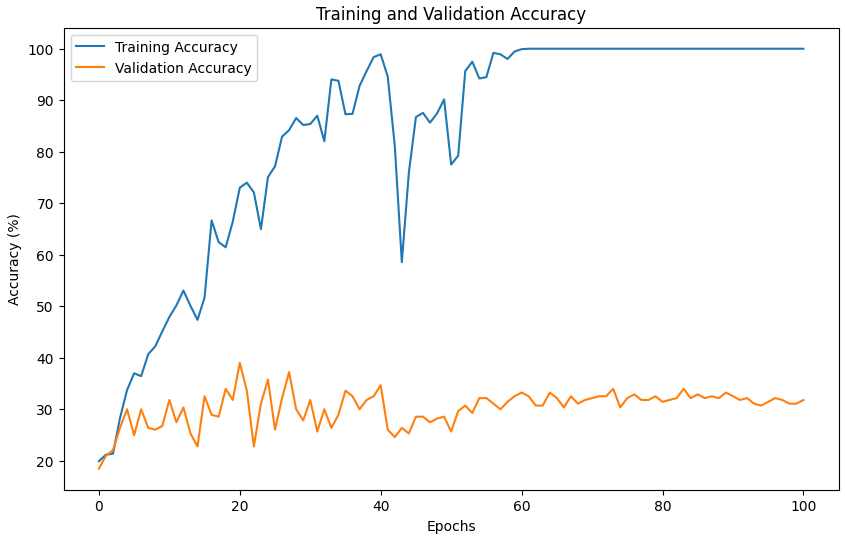
\includegraphics[width=0.8\textwidth]{./figures/task1-accuracy.png}
\caption{Train \& validation accuracies for FFNN}
\label{fig:task1-accuracy}
\end{figure}

\subsection*{7}

Overall, after assessing the performances of the network on the unseen test set
the model is realiable in estimating the classification of the images with
a best accuracy slightly lower of 38.13\% than the best one of the validation set.
The variance of the accuracies is huge: 209.89.
To complement, the Loss averaged is 1.90. 

The delusional and unreliable result is due to the nature of Feed Forward Neural Network:
the learning is focused on pixel per pixel,
while a desired and more useful approach would be the ones resembling human interaction,
i.e. a broad overview of the whole image,
analyzing it in chunks.

As it is difficult for us to spot an image from a puzzle piece,
the FFNN has a metaphorically resembling trouble with image pixels.

For us humans, we might be able to recognize a person (macro-concept) 
from its smile (micro-concept).
A similar concept is the key to improve the results 
and lead to the CNN model approach in Task 2.


\subsection*{8 BONUS}

The bonus was completed with the following features:
the mean and average for each RGB channel.

In Figure (\ref{fig:task1-bonus-accuracy}) 
and Table (\ref{tab:task1-bonus-accuracy}), 
the results show a similar slightly lower accuracy value during training.

\begin{table}[htbp]
\centering
\caption{Training and Validation Accuracy per Epoch for FFNN with features}
\begin{tabular}{ccc}
\toprule
\textbf{Epoch} & \textbf{Train Accuracy (\%)} & \textbf{Validation Accuracy (\%)} \\
\midrule
1    & 19.15  & 20.29  \\
11   & 30.80  & 21.01  \\
21   & 31.89  & 21.74  \\
31   & 32.34  & 25.36  \\
41   & 31.71  & 29.71  \\
51   & 33.60  & 23.91  \\
61   & 33.51  & 31.16  \\
71   & 34.24  & 26.81  \\
81   & 34.06  & 29.71  \\
91   & 34.96  & 29.71  \\
101  & 35.41  & 26.09  \\
\midrule
\multicolumn{3}{c}{Best validation accuracy: 32.61\%} \\
\bottomrule
\end{tabular}
\label{tab:task1-bonus-accuracy}
\end{table}

\begin{figure}[htbp]
\centering
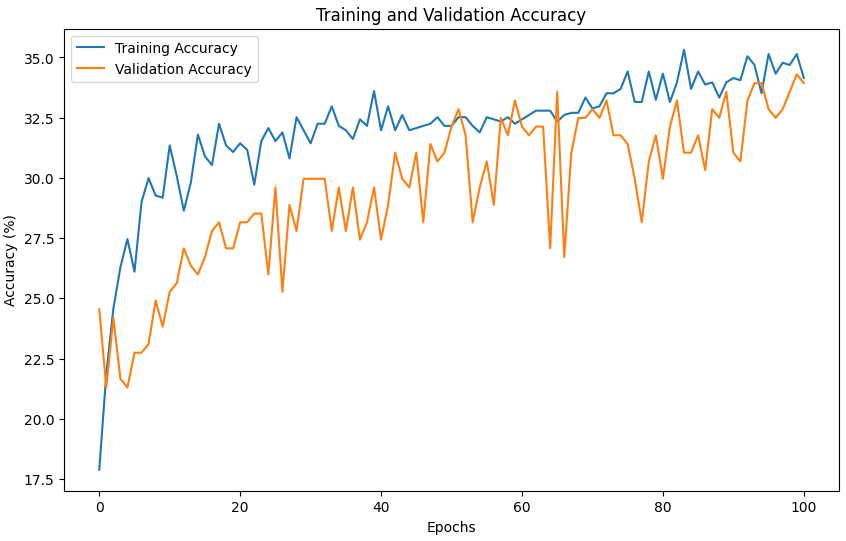
\includegraphics[width=0.8\textwidth]{./figures/task1-bonus-accuracy.png}
\caption{Train \& validation accuracies for FFNN with features}
\label{fig:task1-bonus-accuracy}
\end{figure}

The performance assessment done on the test set 
yields an accuracy of: 35.25\%.
It highlights a slightly lower accuracy 
with respect to the model from T1 with variance of 36.85,
which is far better than the previous model,
but still not enough to be considered reliable for image classification.
To complement, the Loss averaged is 1.58.

Despite more features regarding the image could have been added,
one should be careful to reason about the logical implication of it.
As previously said, the Feed Forward Neural Network 
is not the best model for image classification
due to its nature of pixel per pixel analysis.
Most of these features are not useful for the model to learn from:
althought same type of lions might share the same color of the fur,
most of the proposed felines share a common color palette.

Moreover, the statistical comparison with p-value test set to 
\( p = 0.05 \).
between the FFNN model without features yield 
the following results:
there is \textbf{no statistical significantly difference}. 
The resulted values from statistical comparison are:
\( t\_statistic = -0.15, p\_value = 0.89 \).

It suffers from the same disadvantages from FFNN discussed previously,
so the improvement is sadly bounded by the model nature.

\newpage
%----------------------------------------------------------------------------------------
%	Task 2
%----------------------------------------------------------------------------------------

\section{Image Classification with Convolutional Neural Networks (CNN)}

Implement a multi-class classifier (CNN model) to identify the class of the images: 
'CHEETAH' ,'OCELOT', 'SNOW LEOPARD', 'CARACAL', 'LIONS', 'PUMA', 'TIGER'.

\begin{enumerate}
\item Follow steps 1 and 2 from T1 to prepare the data.

\item Build a CNN of your choice, following these constraints: 

	\begin{itemize}
	\item use 3 convolutional layers.
	\item use 3 pooling layers.
	\item use 3 dense layers (output layer included).
	\end{itemize}

\item Train and validate your model. Choose the right optimizer and loss function. 

\item Follow steps 5 and 6 of T1 to assess performance.

\item Qualitatively and \textbf{statistically} compare the results 
obtained in T1 with the ones obtained in T2. 
Explain what you think the motivations for the difference in performance may be.

\item Apply image manipulation and augmentation techniques in order to improve the performance
of your models. Evaluate the performance of the model using the new images and compare the
results with the previous evaluation performed in part 3. Provide your observations and insights.

\item \textbf{Bonus} (Optional) 
Tune the model hyper-parameters with a \textbf{grid search} 
to improve the performances (if feasible).

	\begin{itemize}
	\item Perform a grid search on the chosen ranges based on hold-out cross-validation 
	in the training set and identify the most promising hyper-parameter setup.

	\item Compare the accuracy on the test set achieved by the most promising configuration 
	with that of the model obtained in point 4. 
	Are the accuracy levels \textbf{statistically} different?
	\end{itemize}
\end{enumerate}

\subsection*{3}

The following train parameters were chosen for the model.
The Optimizer chosen is XXXX because XXXX.
The loss function used is the CrossEntropyLoss function, 
which fits the categorical nature of the classification problem.


\subsection*{4}

In Table (\ref{tab:task2-accuracy}),
the accuracy along the epochs is shown.

In Figure (\ref{fig:task2-accuracy}), 
I provide the plot with epochs on the x-axis where two graphs are plotted:
the train and validation accuracies.
The context is the one from the previous Table (\ref{tab:task2-accuracy}). 

Overall, after assessing the performances of the network on the unseen test set
the model is realiable in estimating the classification of the images with
a best accuracy slightly lower XXX than the one on the validation set,
and the average of the accuracies are around XXX,
with a variance of XXX.

\begin{table}[htbp]
\centering
\caption{Training and Validation Accuracy per Epoch for CNN}
\begin{tabular}{ccc}
\toprule
\textbf{Epoch} & \textbf{Train Accuracy (\%)} & \textbf{Validation Accuracy (\%)} \\
\midrule
1    & 19.15 & 21.30 \\
11   & 97.92 & 64.26 \\
21   & 100.00 & 67.51 \\
31   & 100.00 & 67.51 \\
41   & 100.00 & 67.15 \\
51   & 100.00 & 66.43 \\
61   & 100.00 & 66.43 \\
71   & 100.00 & 67.15 \\
81   & 100.00 & 67.87 \\
91   & 100.00 & 68.59 \\
101  & 100.00 & 68.59 \\
\midrule
\multicolumn{3}{c}{Best validation accuracy: 68.59\%} \\
\bottomrule
\end{tabular}
\label{tab:task2-accuracy}
\end{table}

\begin{figure}[htbp]
\centering
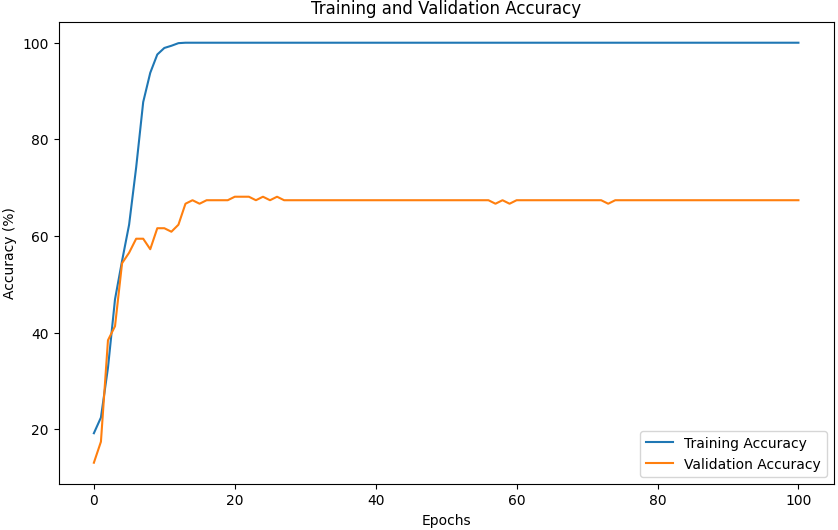
\includegraphics[width=0.8\textwidth]{./figures/task2-accuracy.png}
\caption{Train \& validation accuracies for CNN}
\label{fig:task2-accuracy}
\end{figure}


\subsection*{5}

The statistical comparison between the simple FFNN and the current CNN model yield 
the following results:
there XXXXX statistical significantly difference with the \( p-value = 0.05 \).
The best result is yield by model XXXXX with best accuracy XXXX and variance of XXXX.

\subsection*{6 (present only in README.md)}
\textit{
Apply image manipulation and augmentation techniques in order to improve the performance of your models. 
Evaluate the performance of the model using the new images 
and compare the results with the previous evaluation performed in part 3. 
Provide your observations and insights.
}
In Table (\ref{tab:task2-aug-accuracy}),
the accuracy along the epochs is shown.

In Figure (\ref{fig:task2-aug-accuracy}), 
I provide the plot with epochs on the x-axis where two graphs are plotted:
the train and validation accuracies.
The context is the one from the previous Table (\ref{tab:task2-aug-accuracy}). 

Overall, after assessing the performances of the network on the unseen test set
the model is realiable in estimating the classification of the images with
a best accuracy slightly lower XXX than the one on the validation set,
and the average of the accuracies are around XXX,
with a variance of XXX.

\begin{table}[htbp]
\centering
\caption{Training and Validation Accuracy per Epoch for Augmented CNN}
\begin{tabular}{ccc}
\toprule
\textbf{Epoch} & \textbf{Train Accuracy (\%)} & \textbf{Validation Accuracy (\%)} \\
\midrule
1    & 17.89 & 23.10 \\
11   & 63.23 & 70.40 \\
21   & 78.95 & 79.78 \\
31   & 86.72 & 76.17 \\
41   & 91.96 & 80.51 \\
51   & 95.21 & 79.42 \\
61   & 95.75 & 82.67 \\
71   & 96.21 & 81.23 \\
81   & 96.75 & 80.14 \\
91   & 98.74 & 87.36 \\
101  & 98.19 & 83.03 \\
\midrule
\multicolumn{3}{c}{Best validation accuracy: 87.36\%} \\
\bottomrule
\end{tabular}
\label{tab:task2-aug-accuracy}
\end{table}

\begin{figure}[htbp]
\centering
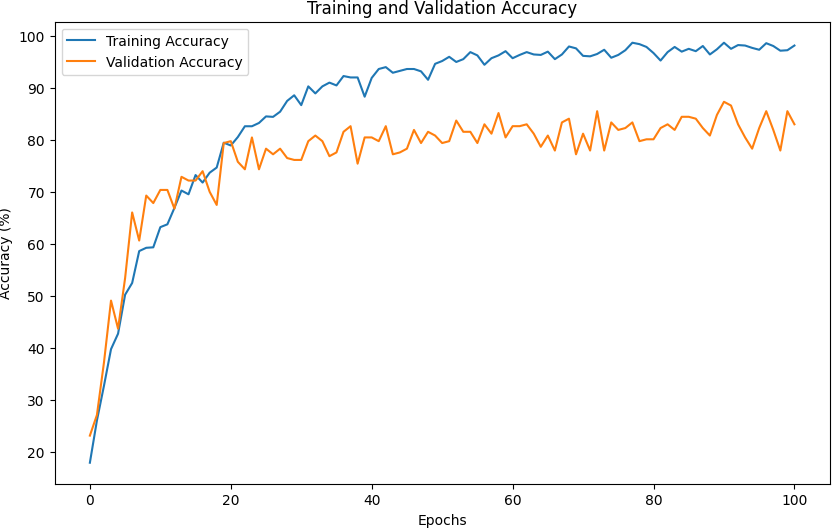
\includegraphics[width=0.8\textwidth]{./figures/task2-aug-accuracy.png}
\caption{Train \& Validation accuracies for Augmented CNN}
\label{fig:task2-aug-accuracy}
\end{figure}


\subsection*{7 BONUS}

For the grid search I choose to change the following hyperparameters:
\begin{itemize}
	\item[1] Learning rate: [0.001, 0.01, 0.1]
	\item[2] Batch size: [32, 64, 128]
	% \item[3] Optimizer: [Adam, SGD]
\end{itemize}

The epochs were fixed at 100 as defined in configuration.

The results of such grid search yield me a model with peak validation accuracy of
\( 62.09 \% \)
with the following best parameters:

\begin{itemize}
	\item batch size = 32
	\item learning rate = 0.001
	\item epochs = 101
\end{itemize}

In Table (\ref{tab:task2-bonus-accuracy}), the accuracy along the epochs is shown.

\begin{table}[htbp]
\centering
\caption{Training and Validation Accuracy per Epoch for CNN with Grid Search}
\begin{tabular}{ccc}
\toprule
\textbf{Epoch} & \textbf{Train Accuracy (\%)} & \textbf{Validation Accuracy (\%)} \\
\midrule
1    & 21.05 & 27.44 \\
11   & 99.01 & 53.07 \\
21   & 100.00 & 66.43 \\
31   & 100.00 & 66.06 \\
41   & 100.00 & 65.34 \\
51   & 100.00 & 65.34 \\
61   & 100.00 & 65.34 \\
71   & 100.00 & 66.06 \\
81   & 100.00 & 66.43 \\
91   & 100.00 & 66.79 \\
101  & 100.00 & 66.06 \\
\midrule
\multicolumn{3}{c}{Best validation accuracy: 67.15\%} \\
\bottomrule
\end{tabular}
\label{tab:task2-bonus-accuracy}
\end{table}


\newpage
%----------------------------------------------------------------------------------------
%	Task 3
%----------------------------------------------------------------------------------------
\section{Transfer Learning}

This task involves loading the VGG19 model from PyTorch, 
applying transfer learning, and experimenting with different model cuts. 
The VGG19 architecture have 19 layers grouped into 5 blocks, 
comprising 16 convolutional layers followed by 3 fully-connected layers. 
Its success in achieving strong performance on various image classification benchmarks 
makes it a well-known model.

Your task is to apply transfer learning with a pre-trained VGG19 model. 
A code snippet that loads the VGG19 model from PyTorch is provided. 
You'll be responsible for completing the remaining code sections (marked as TODO). 
Specifically:

\begin{enumerate}
    \item The provided code snippet sets param.requires\_grad = False 
	for the pre-trained VGG19 model's parameters. 
	Can you explain the purpose of this step in the context of transfer learning and fine-tuning? 
	Will the weights of the pre-trained VGG19 model be updated during transfer learning training?

    \item We want to transfer learning with a pre-trained VGG19 model 
	for our specific classification task. The code has sections for \_\_init\_\_ 
	and forward functions but needs to be completed to incorporate two different "cuts" 
	from the VGG19 architecture. 
	After each cut, additional linear layers are needed for classification 
	(similar to Block 6 of VGG19).
	Implement the \_\_init\_\_ and forward functions to accommodate these two cuts:

	\begin{itemize}
		\item This cut should take the pre-trained layers up to 
		and including the 11th convolution layer (Block 4).

		\item Cut 2: This cut should use all the convolutional layers 
		from the pre-trained VGG19 model (up to Block 5).
		
		Note after each cut take the activation function and the pooling layer 
		associated with the convolution layer on the cut

		\begin{figure}[th]
			\centering
			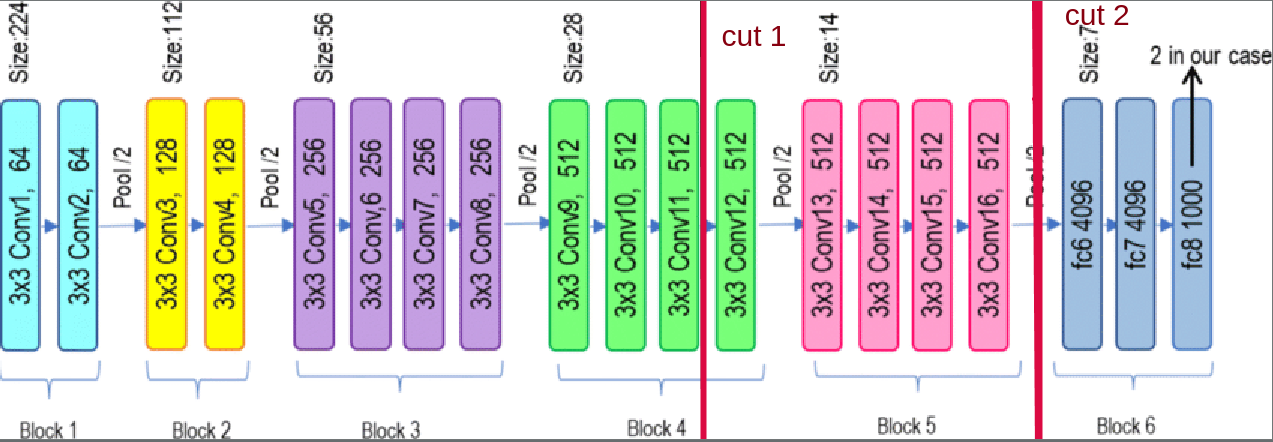
\includegraphics[scale=0.33]{cuts.png}
			\caption{Cuts in VGG19}
			\label{fig:model-vgg19}
		\end{figure}
	\end{itemize}

	\item In both cases, after the cut, add a sequence of layers (of your choice) 
	with appropriate activation functions, leading to a final output layer 
	with the desired number of neurons for your classification task.
	Train the two models (one with Cut 1 and another with Cut 2) on your chosen dataset. 
	Once training is complete, compare their performance statistically.

	\item Based on the performance comparison, 
	discuss any observed differences between the two models. 
	What could be the potential reasons behind these results?

	\item BONUS (optional): Try different cuts in each block of VGG19, 
	and plot one single figure with all the train-validation-test accuracies. 
	Explain in detail the reasons behind the variation of results you get.
\end{enumerate}


\subsection*{1}

Within the context of transfer learning, the model VGG19 from PyTorch 
is loaded with the architecture and weights of a pre-trained model.
The purpose of setting \pyth{param.requires_grad = False} 
is to \textbf{freeze the weights} of the model,
so that the model does not update the weights during the training of the new model.
In fact, it would not make sense to update the weights of the pre-trained model
in the context of transfer learning.
Particularly, transfer learning is a tecnique where a model for one task,
in this case the VGG19 for image classification, 
is reused as the starting point for a model on a second task,
where the fine tuning to train the model over our feline dataset happens.
Hence, during transfer learning traning, 
the weights of the pre-trained VGG19 will XXX be updated.


\subsection*{2}

To select the first cut, we need to from the firt feature children of the 
VGG19 architecture to index 25, in order to get the 11th convolution layer 
and its activation function and pooling layers associated.
The correctness can be easily checked thanks to the already templated 
\pyth{print(self.features)}
after the cut, so you will see all the requirements satisfied.

For the second cut, we trivially load all the features from the model.


\subsection*{3}

For fine tuning we put also a sequence of 3 linear layers 
with relu activation function complementing 
with a dropout strategy to try to avoid overfitting.
Starting from flattened image size on the VGG19,
for which I wrote a dummy input in the constructor to retrieve what would be the
flatten image after the features of the pre-trained model up to its 11th convolution
layer and its associated activation functions and pools for cut1.
The number of neuron in the added sequence of layers were 256 and 128, 
ending with an output correspoding to our cat types in the dataset, i.e. 6.

In Table (\ref{tab:task3-cut1-accuracy}),
the accuracy along the epochs is shown.

In Figure (\ref{fig:task3-cut1-accuracy}), 
I provide the plot with epochs on the x-axis where two graphs are plotted:
the train and validation accuracies.
The context is the one from the previous Table (\ref{tab:task3-cut1-accuracy}). 

Overall, after assessing the performances of the network on the unseen test set
the model is realiable in estimating the classification of the images with
a best accuracy slightly lower XXX than the one on the validation set,
and the average of the accuracies are around XXX,
with a variance of XXX.

\begin{table}[htbp]
\centering
\caption{Training and Validation Accuracy per Epoch for fine-tuned VGG19 with Cut 1}
\begin{tabular}{ccc}
\toprule
\textbf{Epoch} & \textbf{Train Accuracy (\%)} & \textbf{Validation Accuracy (\%)} \\
\midrule
1    & 33.79 & 71.84 \\
11   & 67.66 & 79.42 \\
21   & 78.77 & 85.20 \\
31   & 81.93 & 83.03 \\
41   & 82.84 & 81.95 \\
51   & 84.10 & 83.75 \\
61   & 85.00 & 83.75 \\
71   & 87.08 & 87.00 \\
81   & 86.54 & 83.75 \\
91   & 85.82 & 84.84 \\
101  & 86.27 & 89.53 \\
\midrule
\multicolumn{3}{c}{Best validation accuracy: 89.53\%} \\
\bottomrule
\end{tabular}
\label{tab:task3-cut1-accuracy}
\end{table}


\begin{figure}[htbp]
\centering
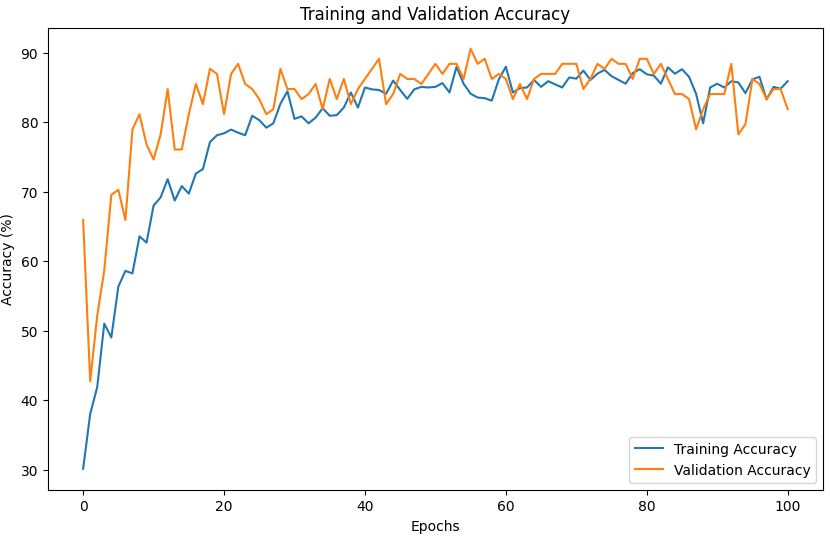
\includegraphics[width=0.8\textwidth]{./figures/task3-cut1-accuracy.png}
\caption{Train \& validation accuracies for fine-tuned VGG19 with Cut 1}
\label{fig:task3-cut1-accuracy}
\end{figure}


In Table (\ref{tab:task3-cut2-accuracy}),
the accuracy along the epochs is shown.

In Figure (\ref{fig:task3-cut2-accuracy}), 
I provide the plot with epochs on the x-axis where two graphs are plotted:
the train and validation accuracies.
The context is the one from the previous Table (\ref{tab:task3-cut2-accuracy}). 

Overall, after assessing the performances of the network on the unseen test set
the model is realiable in estimating the classification of the images with
a best accuracy slightly lower XXX than the one on the validation set,
and the average of the accuracies are around XXX,
with a variance of XXX.

\begin{table}[htbp]
\centering
\caption{Training and Validation Accuracy per Epoch for fine-tuned VGG19 with Cut 2}
\begin{tabular}{ccc}
\toprule
\textbf{Epoch} & \textbf{Train Accuracy (\%)} & \textbf{Validation Accuracy (\%)} \\
\midrule
1    & 61.52 & 93.14 \\
11   & 98.92 & 95.31 \\
21   & 99.01 & 97.11 \\
31   & 98.37 & 91.34 \\
41   & 99.73 & 94.22 \\
51   & 99.46 & 94.58 \\
61   & 99.64 & 93.86 \\
71   & 99.82 & 93.50 \\
81   & 99.37 & 95.67 \\
91   & 99.28 & 94.58 \\
101  & 99.37 & 94.58 \\
\midrule
\multicolumn{3}{c}{Best validation accuracy: 97.11\%} \\
\bottomrule
\end{tabular}
\label{tab:task3-cut2-accuracy}
\end{table}

\begin{figure}[htbp]
\centering
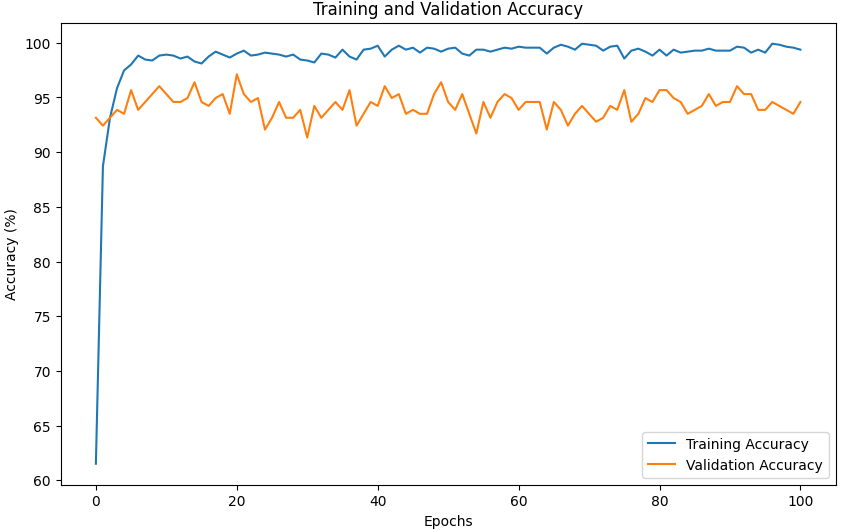
\includegraphics[width=0.8\textwidth]{./figures/task3-cut2-accuracy.png}
\caption{Train \& validation accuracies for fine-tuned VGG19 with Cut 2}
\label{fig:task3-cut2-accuracy}
\end{figure}


The statistical comparison 
between the cut1 and the cut2 pre-trained and fine-tuned models yield 
the following results:
there XXXXX statistical significantly difference with the \( p-value = 0.05 \).
The best result is yield by model XXXXX with best accuracy XXXX and variance of XXXX.

\subsection*{4}

Based on the performance comparison, 
the reason why the cut 2 performs significantly better than cut 1
lies within the transfer learning of the VGG19 itself:
its architecture is meant to be used XXXX.

Hence, the potential reason of the lower accuracy for cut 1 
woud be indeed in the difference of XXX.

\subsection*{5 BONUS}

For the bonus part, I chose the following different cuts among the blocks
of the VGG19 model:

\begin{itemize}
	\item \textbf{Cut A} only first block
	\item \textbf{Cut B} 2 blocks
	\item \textbf{Cut C} 3 blocks
	\item \textbf{Cut D} 4 blocks
	\item \textbf{Cut E} 5 blocks
\end{itemize}

In Figures (\ref{fig:task3-bonus-histogram}, \ref{fig:task3-bonus-plot}), 
the result plot of the train-test-validation of accuracies are presented 
in two flavours respectively:
an histogram and a line plot.

\begin{figure}[htbp]
	\centering
	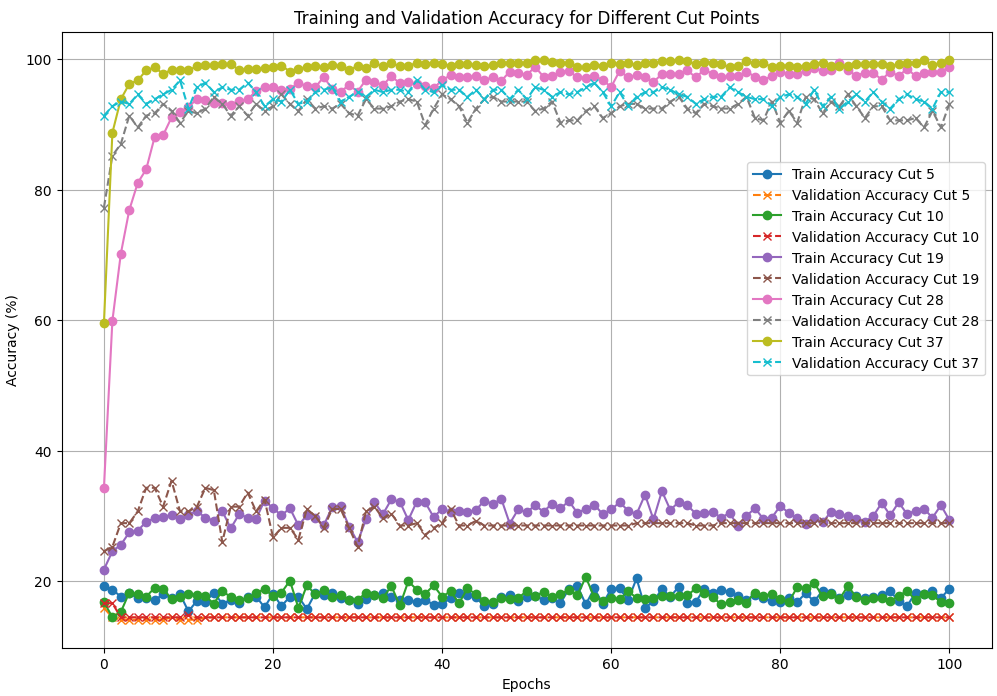
\includegraphics[width=\textwidth]{task3-bonus-plot.png}
	\caption{train-test-validation accuracies plot}
	\label{fig:task3-bonus-plot}
\end{figure}

\begin{figure}[htbp]
	\centering
	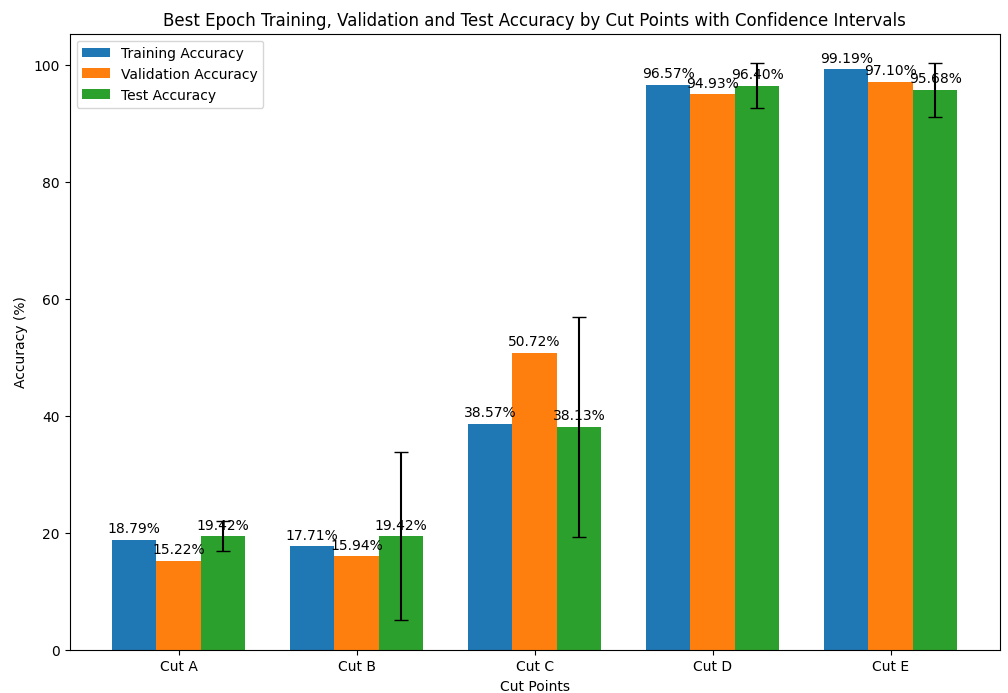
\includegraphics[width=0.8\textwidth]{task3-bonus-histogram.png}
	\caption{train-test-validation accuracies histogram}
	\label{fig:task3-bonus-histogram}
\end{figure}

The reason behind such variation of results leads to a stronger 
support of the previously mentioned difference between cut1 and cut2:
XXXXXX.

Time increases with layers, it makes sense to choose fewer sufficient layers.

In Tables (
	\ref{tab:task3-bonus-cuta-accuracy},
	\ref{tab:task3-bonus-cutb-accuracy},
	\ref{tab:task3-bonus-cutc-accuracy},
	\ref{tab:task3-bonus-cutd-accuracy},
	\ref{tab:task3-bonus-cute-accuracy}
),the accuracies for respectively
for Cut A, B, C, D, E are showcased.

\begin{table}[htbp]
\centering
\caption{Training and Validation Accuracy per Epoch for Model Cut A}
\begin{tabular}{ccc}
\toprule
\textbf{Epoch} & \textbf{Train Accuracy (\%)} & \textbf{Validation Accuracy (\%)} \\
\midrule
1    & 19.24 & 15.88 \\
11   & 15.36 & 14.08 \\
21   & 18.07 & 14.44 \\
31   & 16.53 & 14.44 \\
41   & 16.53 & 14.44 \\
51   & 17.52 & 14.44 \\
61   & 18.79 & 14.44 \\
71   & 16.80 & 14.44 \\
81   & 16.80 & 14.44 \\
91   & 17.43 & 14.44 \\
101  & 18.79 & 14.44 \\
\midrule
\multicolumn{3}{c}{Best validation accuracy: 15.88\%} \\
\bottomrule
\end{tabular}
\label{tab:task3-bonus-cuta-accuracy}
\end{table}

\begin{table}[htbp]
\centering
\caption{Training and Validation Accuracy per Epoch for Model Cut B}
\begin{tabular}{ccc}
\toprule
\textbf{Epoch} & \textbf{Train Accuracy (\%)} & \textbf{Validation Accuracy (\%)} \\
\midrule
1    & 16.80 & 16.61 \\
11   & 17.98 & 14.80 \\
21   & 17.71 & 14.44 \\
31   & 17.16 & 14.44 \\
41   & 17.62 & 14.44 \\
51   & 18.52 & 14.44 \\
61   & 17.34 & 14.44 \\
71   & 18.88 & 14.44 \\
81   & 17.25 & 14.44 \\
91   & 17.16 & 14.44 \\
101  & 16.62 & 14.44 \\
\midrule
\multicolumn{3}{c}{Best validation accuracy: 16.61\%} \\
\bottomrule
\end{tabular}
\label{tab:task3-bonus-cutb-accuracy}
\end{table}

\begin{table}[htbp]
\centering
\caption{Training and Validation Accuracy per Epoch for Model Cut C}
\begin{tabular}{ccc}
\toprule
\textbf{Epoch} & \textbf{Train Accuracy (\%)} & \textbf{Validation Accuracy (\%)} \\
\midrule
1    & 21.77 & 24.55 \\
11   & 30.17 & 30.69 \\
21   & 31.17 & 26.71 \\
31   & 26.02 & 25.27 \\
41   & 31.07 & 28.88 \\
51   & 30.53 & 28.52 \\
61   & 30.98 & 28.52 \\
71   & 30.35 & 28.52 \\
81   & 31.53 & 28.88 \\
91   & 29.09 & 28.88 \\
101  & 29.36 & 28.88 \\
\midrule
\multicolumn{3}{c}{Best validation accuracy: 35.38\%} \\
\bottomrule
\end{tabular}
\label{tab:task3-bonus-cutc-accuracy}
\end{table}

\begin{table}[htbp]
\centering
\caption{Training and Validation Accuracy per Epoch for Model Cut D}
\begin{tabular}{ccc}
\toprule
\textbf{Epoch} & \textbf{Train Accuracy (\%)} & \textbf{Validation Accuracy (\%)} \\
\midrule
1    & 34.24 & 77.26 \\
11   & 92.59 & 92.06 \\
21   & 95.66 & 92.78 \\
31   & 95.03 & 91.34 \\
41   & 96.75 & 94.58 \\
51   & 97.56 & 93.50 \\
61   & 95.75 & 91.70 \\
71   & 97.20 & 91.70 \\
81   & 98.10 & 90.25 \\
91   & 97.92 & 90.97 \\
101  & 98.74 & 93.14 \\
\midrule
\multicolumn{3}{c}{Best validation accuracy: 94.58\%} \\
\bottomrule
\end{tabular}
\label{tab:task3-bonus-cutd-accuracy}
\end{table}

\begin{table}[htbp]
\centering
\caption{Training and Validation Accuracy per Epoch for Model Cut E}
\begin{tabular}{ccc}
\toprule
\textbf{Epoch} & \textbf{Train Accuracy (\%)} & \textbf{Validation Accuracy (\%)} \\
\midrule
1    & 59.53 & 91.34 \\
11   & 98.28 & 92.42 \\
21   & 98.74 & 93.86 \\
31   & 98.92 & 94.95 \\
41   & 99.19 & 96.03 \\
51   & 99.46 & 93.86 \\
61   & 99.37 & 92.78 \\
71   & 99.19 & 93.14 \\
81   & 99.01 & 94.22 \\
91   & 99.28 & 93.50 \\
101  & 99.82 & 94.95 \\
\midrule
\multicolumn{3}{c}{Best validation accuracy: 96.75\%} \\
\bottomrule
\end{tabular}
\label{tab:task3-bonus-cute-accuracy}
\end{table}


\end{document}
